\documentclass{article}
\usepackage[utf8]{inputenc}
\usepackage{tikz, pgfplots}
\usetikzlibrary{positioning}
\title{tikz}
\author{marajul haque}

\begin{document}
	\maketitle
	
	\section{TikZ}
	
	\tikz \draw[very thick][red] [->](0,0)--(2,1)--(3,2);
	
	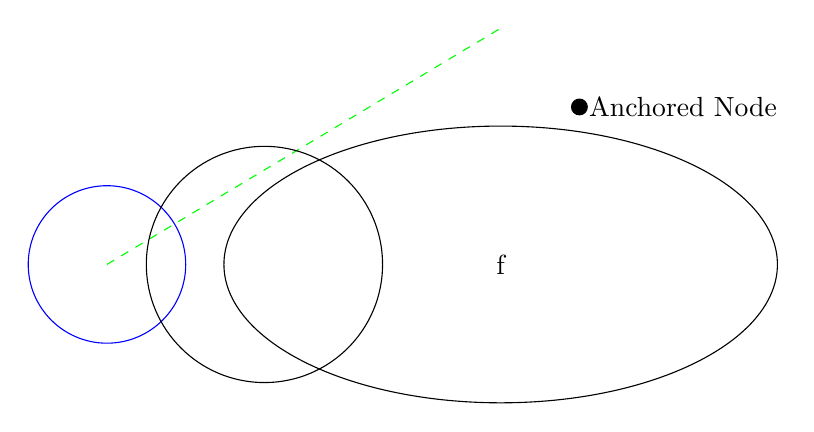
\begin{tikzpicture} 
		
		\draw[dashed][red,blue,green] (0,0)--(5,3);
		
		\draw[red,blue] (0,0) circle(1);
		\draw (2,0) circle(1.5);
		\draw (5,0) ellipse(100pt and 50pt);
		\draw node at (5,0) {f};
		\filldraw (6,2) circle(.1cm) node [anchor=west]{Anchored Node};
	
	\end{tikzpicture}
	
	\vspace{1in}
	
	
	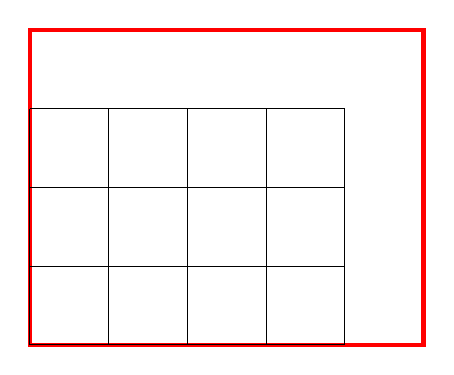
\begin{tikzpicture}
		\draw [ultra thick][red] (0,0) rectangle(5,4);
		\draw (0,0) grid(4,3);
		
	\end{tikzpicture}
	
	\vspace{10in}
	
	\begin{center}
		
		
\begin{tikzpicture} [transform canvas={scale=4.0}]

\draw [blue] (0,1) arc(90:-90:.5cm and 1cm);

\draw [dashed] (0,1) arc (90:270:.5cm and 1cm);

\draw (0,0) circle(1cm);
\filldraw [red] (0,1) circle (0.05);
\filldraw [red] (0,-1) circle(0.05);


\shade [ball color = blue!10!red,opacity=.50] (0,0) circle(1cm);



		
			
		\end{tikzpicture}
	\end{center}
	
	\vspace{11in}
	\begin{center}
	

	
	
\begin{tikzpicture}[transform canvas={scale=2}]
		
		\draw[dashed] [red] (0,0) circle(2);
		
		%\filldraw[red] (0,0) rectangle(4,4);
		
		\draw (0,0) circle(.1cm) node[anchor=north]{center};
		
\shade [ball color =red!50!yellow,opacity=.5](0,0) rectangle(2,2);
		
	
	\end{tikzpicture}
		\end{center}
		
		
		\vspace{10in}
		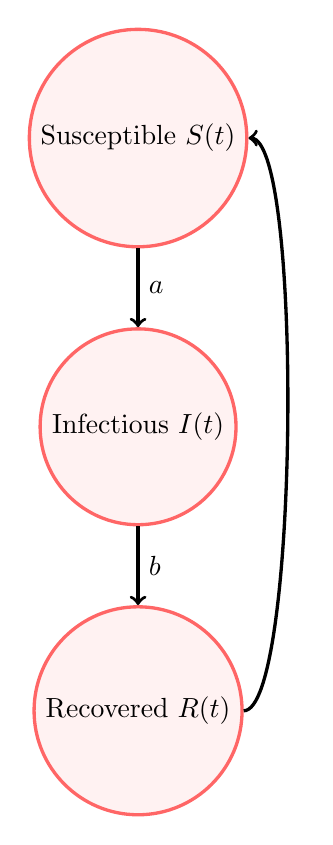
\begin{tikzpicture}	[SI/.style={circle, draw=red!60, fill=red!5, very thick, minimum size =5mm},
 		]
		
		
		\node[SI] (Susceptible)                       {Susceptible $S(t)$};
		\node[SI] (Infectious)  [below=of Susceptible] {Infectious $I(t)$};
	\node[SI] (Recovered) [below= of Infectious ] {Recovered $R(t)$};
	
	
	
	
	\draw [->, very thick] (Susceptible.south) to node[right] {$a$}(Infectious.north);
	\draw [->, very thick] (Infectious.south) to node[right] {$b$} (Recovered.north);
	\draw [->, very thick] (Recovered.east) .. controls + (right:7mm) and +(right:7mm)	.. (Susceptible.east);
	
	
	
	
		\end{tikzpicture}
		
		
		
		
		
	
\end{document}